\chapter{Malla curricular}\label{chap:GeneralInfo}

\section{Clasificación de los cursos por niveles}
De acuerdo a la \textit{Computing Curricula}, los cursos son clasificados en 3 niveles: 
Introductorios, Intermedios y Avanzados como puede ser observado en la Figura \ref{fig:niveles}. 
Los abordajes posibles para iniciar una carrera de este tipo de acuerdo al estándar son: 
Imperativo, Objetos, Funcional, Visión amplia, Algoritmos, Hardware.
 
Los cursos de nivel intermedio pueden tener las siguientes orientaciones: 
Basado en tópicos, comprimido, basado en sistemas, orientado a la internet. 
Los cursos de tercer nivel tienen por objetivo abrir varias posibilidades de 
especialización por lo que no están divididos en categorí­as.

\begin{figure}[ht]
   \centering
   \includegraphics[width=13cm]{\OutputFigsDir/course-levels}
   \caption{Orientaciones de los cursos por niveles.}
   \label{fig:niveles}
\end{figure}

Esta propuesta de malla curricular está basada en el abordaje funcional en el nivel introductorio y orientado 
a internet en el nivel intermedio. El abordaje funcional fue escogido porque nos da la oportunidad de 
concentrarnos en el desarrollo algoritmico del alumno y no en el aprendizaje de sintaxis de un lenguaje 
en particular. El abordaje orientado a la web se escogió porque hacia eso apuntan las 
tendencias futuras de la computación.

\section{Codificación de los cursos}
Los cursos se encuentran codificados bajo el esquema que se muestra en la Figura~\ref{fig:course-coding}:
\begin{figure}[ht]
   \centering
    \psframebox[fillstyle=solid,fillcolor=white]{ 
      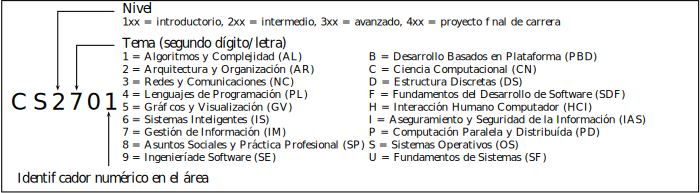
\includegraphics[width=13cm]{\OutputFigsDir/course-coding} 
     }
   \caption{Esquema de codificación para los cursos de Sistemas de Información y Tecnologí­a de la Información.}
   \label{fig:course-coding}
\end{figure}

% TODO: Ruta para CS esta no generalizada.     
\begin{figure}[ht]
   \centering
%    \psframebox[fillstyle=solid,fillcolor=white]{ 
      \includegraphics[width=13cm]{\OutputFigsDir/CS-course-coding} 
% 	}
   \caption{Esquema de codificación para los cursos para los cursos de Ciencia de la Computación.}
   \label{fig:cs-course-number}
\end{figure}

El área de un curso está determinada por sus 2 primeras letras. Los posibles códigos para estas lí­neas son:
% TODO areas-description is missing
% \input{\OutputTexDir/areas-description}

\begin{landscape}
\section{Malla curricular por semestres}\label{sec:courses-by-semester}
La relación de cursos se muestra a continuación:
% TODO tables-by-semester
%\input{\OutputTexDir/tables-by-semester}

\OnlySPC{Es importante resaltar que todos los semestres podrí­an ser completados con cursos extras de acuerdo al perfil de la institución.}
\end{landscape}

\section{Estadí­sticas de la malla curricular}
Esta propuesta puede ser analizada por el número de créditos dedicados a cada área )(Fig.~\ref{fig:pie-credits}) %horas de clase de las mismas 
y por niveles de cursos (Introductorios, Intermedios, Avanzados y Proyectos) (Fig.~\ref{fig:pie-by-levels}).

\vspace{0.5cm}
\begin{figure}[h!]
      \centering
      \includegraphics[width=10cm]{\OutputFigsDir/pie-credits}
      \label{fig:pie-credits}
      \caption{Distribución de cursos por áreas considerando creditaje.}
\end{figure}

\begin{figure}[h!]
      \centering
      \includegraphics[width=10cm]{\OutputFigsDir/pie-by-levels}
      \label{fig:pie-by-levels}
      \caption{Distribución de créditos por niveles de cursos.}
\end{figure}

\begin{landscape}
\section{Visión gráfica de la Malla curricular}\label{sec:graphic-small-curricula}
\vspace{-0.3cm}Este documento también puede ser analizado desde el punto de vista de los 
prerequisitos de forma gráfica (Fig.~\ref{fig:graphic-small-curricula}).

% TODO
%\begin{figure}[h!]
%	\includegraphics[width=23cm,height=13cm]{\OutputFigsDir/small-graph-curricula.ps}
%	\label{fig:graphic-small-curricula}
%	\caption{Malla curricular \SchoolFullName}
%\end{figure}
\end{landscape}

\section{Compatibilidad de la carrera con relación a estandares internacionales}
En esta sección presentamos la distribución de cursos por áreas de concentración en 
contraste con las propuestas internacionales de las carreras de la \textit{Computing Curricula} 
de IEEE-CS/ACM.

Es necesario notar que \underline{en algunos casos las materias podrí­an aparecen en más de un eje} 
pues tienen contenido de más de una área. 
Por ejemplo, la materia de sistemas operativos contiene unidades de aplicación 
que pueden ser clasificadas en Tecnologí­a de Información pero al mismo tiempo contiene fundamentos 
de como está estructurado un Sistema Operativo que es del eje de Ciencia de la Computación. 
En estos casos el creditaje ha sido divido entre los ejes correspondientes.
% TODO 
%\input{\OutputTexDir/list-of-courses-per-area}

Considerando esta distribución, las figuras \ref{fig:comparing-curves-\currentarea-\currentinstitution-with-CE} 
a la \ref{fig:comparing-curves-\currentarea-\currentinstitution-with-SE} 
nos permiten tener una visión gráfica de esta malla curricular frente a las propuestas de 
carreras presentadas por IEEE-CS/ACM en la \textit{Computing Curricula}

% TODO
%\input{\OutputTexDir/comparing-with-standards}

%\begin{landscape}
%\section{Distribución de tópicos por curso}\label{sec:topics-by-course}
Las siguientes tablas nos muestran la distribución de todos los tópicos del 
cuerpo del conocimiento de \ac{\currentarea} en todos los cursos.
\section{Distribución de tópicos por curso}\label{sec:topics-by-course}
Las siguientes tablas nos muestran la distribución de todos los tópicos del 
cuerpo del conocimiento de \ac{\currentarea} en todos los cursos.
\section{Distribución de tópicos por curso}\label{sec:topics-by-course}
Las siguientes tablas nos muestran la distribución de todos los tópicos del 
cuerpo del conocimiento de \ac{\currentarea} en todos los cursos.
\input{\OutputTexDir/topics-by-course}
%\end{landscape}

%\begin{landscape}
%\section{Resultados esperados distribuí­dos por curso}\label{sec:outcomes-by-course}
Las siquientes tablas nos muestras una visión global de los resultados que se esperan lograr en cada 
curso de la presente malla curricular. 
La lista completa de resultados esperados se encuentra en la Sección:~\ref{sec:outcomes}.
\input{\OutputTexDir/outcomes-by-course-\LANG}
%\end{landscape}
